\section{Architecture du projet}

\subsection{Un système client/serveur}

Au premier semestre de cette année, notre étude bibliographique nous a permis d'étudier les deux systèmes de fenêtrage majeurs sous Linux : X Window System (implémentation X.Org) et le tout jeune Wayland.
Cette étude nous a permis de décider de nous inspirer de X Window System pour l'implémentation de notre système de fenêtrage : nous l'avons trouvé à la fois élégant et adapté à nos objectifs.
De plus, l'implémentation X.Org étant un projet mûr, il est très bien documenté et les solutions conceptuelles qu'il a utilisé sont validées et fonctionnent.

Notre système de fenêtrage est donc divisé en deux grandes parties : le serveur graphique en tant que tel, Pron, et la librairie client implémentant le protocole de communication, la Pronlib.
Après avoir étudié les solutions existantes pour ce qui est de la gestion des fenêtres, nous avons opté pour un système inspiré de Metacity.
Le gestionnaire de fenêtres, Guacamole, est donc un client du serveur graphique à part entière et intercepte certains événements comme on le verra à la section \ref{Guacamole}.
Enfin, la librairie de widgets, Sombrero, s'inspire à la fois de Qt (en version 4) et de gtkmm (wrapper pour GTK+).

Voici un schéma illustrant les différents acteurs de notre architecture et leurs dépendances.
On peut voir que la Pronlib est le cœur de notre système.
Elle est utilisée par tous les éléments pour communiquer avec Pron, et Pron utilise également les structures qu'elle définit pour communiquer avec ses clients (c'est dans la Pronlib que se trouvent toutes les types correspondant au protocole de communication).
  
\begin{figure}[H]
  \centering
  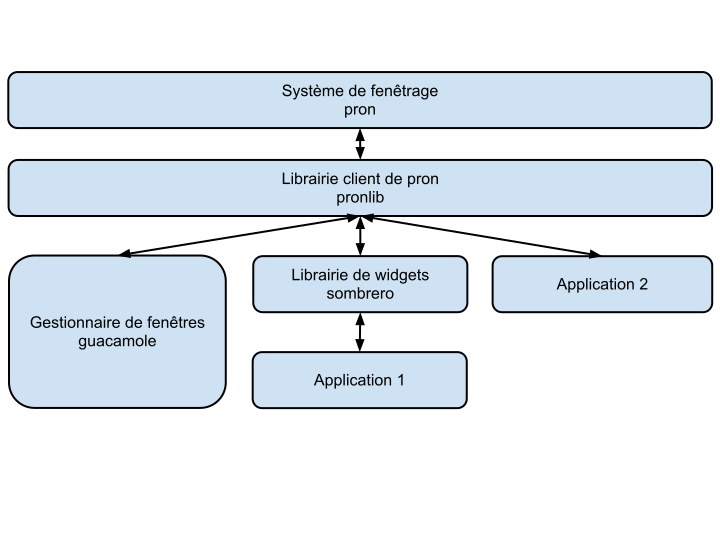
\includegraphics[width=14cm]{images/architecture.png}
  \caption{Architecture}
  \label{fig:architecture}
\end{figure}

On remarque que Guacamole utilise directement la PronLib.
C'est toujours le cas au moment de la rédaction de ce rapport, mais il sera bientôt réimplémenté avec la librairie de widgets Sombrero.

\subsection{Langage de programmation}

Pour ce projet, nous avons décidé d'utiliser le C++ pour de nombreuses raisons :

\begin{itemize}
  \item Langage orienté objet : la COO\footnote{Conception Orientée Objet} est très agréable, notamment pour une librairie de widgets
  \item Langage compilé : pas besoin d'environnement d'exécution comme Java qui n'est pas disponible sous TacOS
  \item Facile à intégrer à un projet en C (TacOS étant codé en C)
  \item Performances
  \item Langage connu et apprécié par les membres de l'équipe
  \item Langage offrant à la fois des fonctionnalités de bas niveau et de haut niveau
  \item Langage permettant l'héritage multiple
\end{itemize}
